\section{Results}

\subsection{City coverage and uncertainty outputs}

Table~\ref{tab:city-coverage} shows the frozen city-level summary for the four inference cities. By construction, the calibrated median surface sums to the official total in every city. What differs is the uncertainty burden and the distribution of confidence bands. Almaty has the lowest median relative uncertainty among the four freeze cities (0.170) together with the largest high-confidence share (22.9\%). Semey has the heaviest median relative uncertainty burden (0.349), but still retains a small high-confidence subset (3.4\%). Astana and Shymkent have no high-confidence share in the frozen city-level summary and therefore should be interpreted more cautiously as screening surfaces.

\input{tables_tex/table1_v3_city_coverage.tex}

Figure~\ref{fig:uncertainty-output} shows two complementary views of the same pattern: an Almaty example of calibrated median proxy value versus relative uncertainty, and the city-level distribution of median relative uncertainty. The figure makes clear that uncertainty is not spatially uniform even within the strongest freeze-city case.

\begin{figure}[H]
\centering
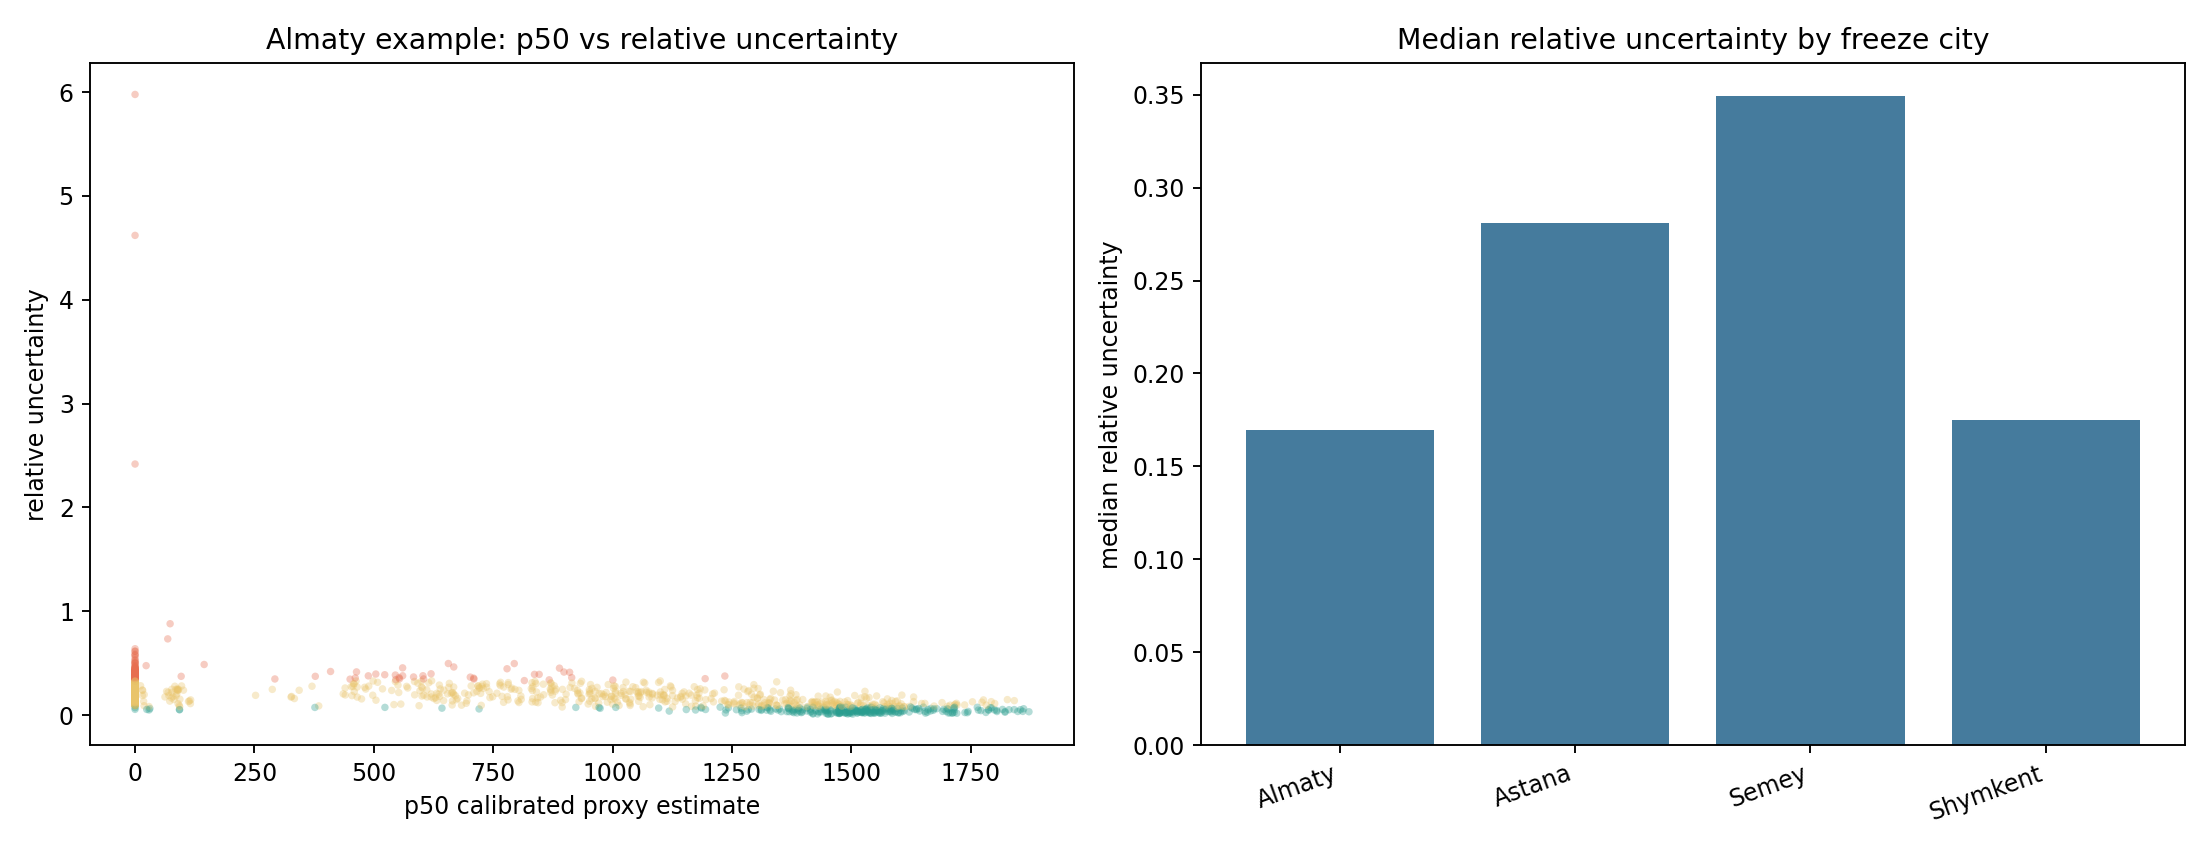
\includegraphics[width=\textwidth]{figures/fig2_uncertainty_output_example.png}
\caption{Uncertainty output summary from the frozen four-city package. Left: Almaty cell-level calibrated median proxy estimates against relative uncertainty. Right: median relative uncertainty by freeze city. This figure shows that uncertainty burden varies within and across cities; it does not validate true census uncertainty.}
\label{fig:uncertainty-output}
\end{figure}

Figure~\ref{fig:confidence-distribution} shows how confidence bands distribute across cities. Almaty is the only city with a substantial high-confidence share, Semey retains a small high-confidence slice, and Astana and Shymkent are dominated by medium and low bands. This is consistent with the intended v3 interpretation: not every city supports the same level of screening confidence.

\begin{figure}[H]
\centering
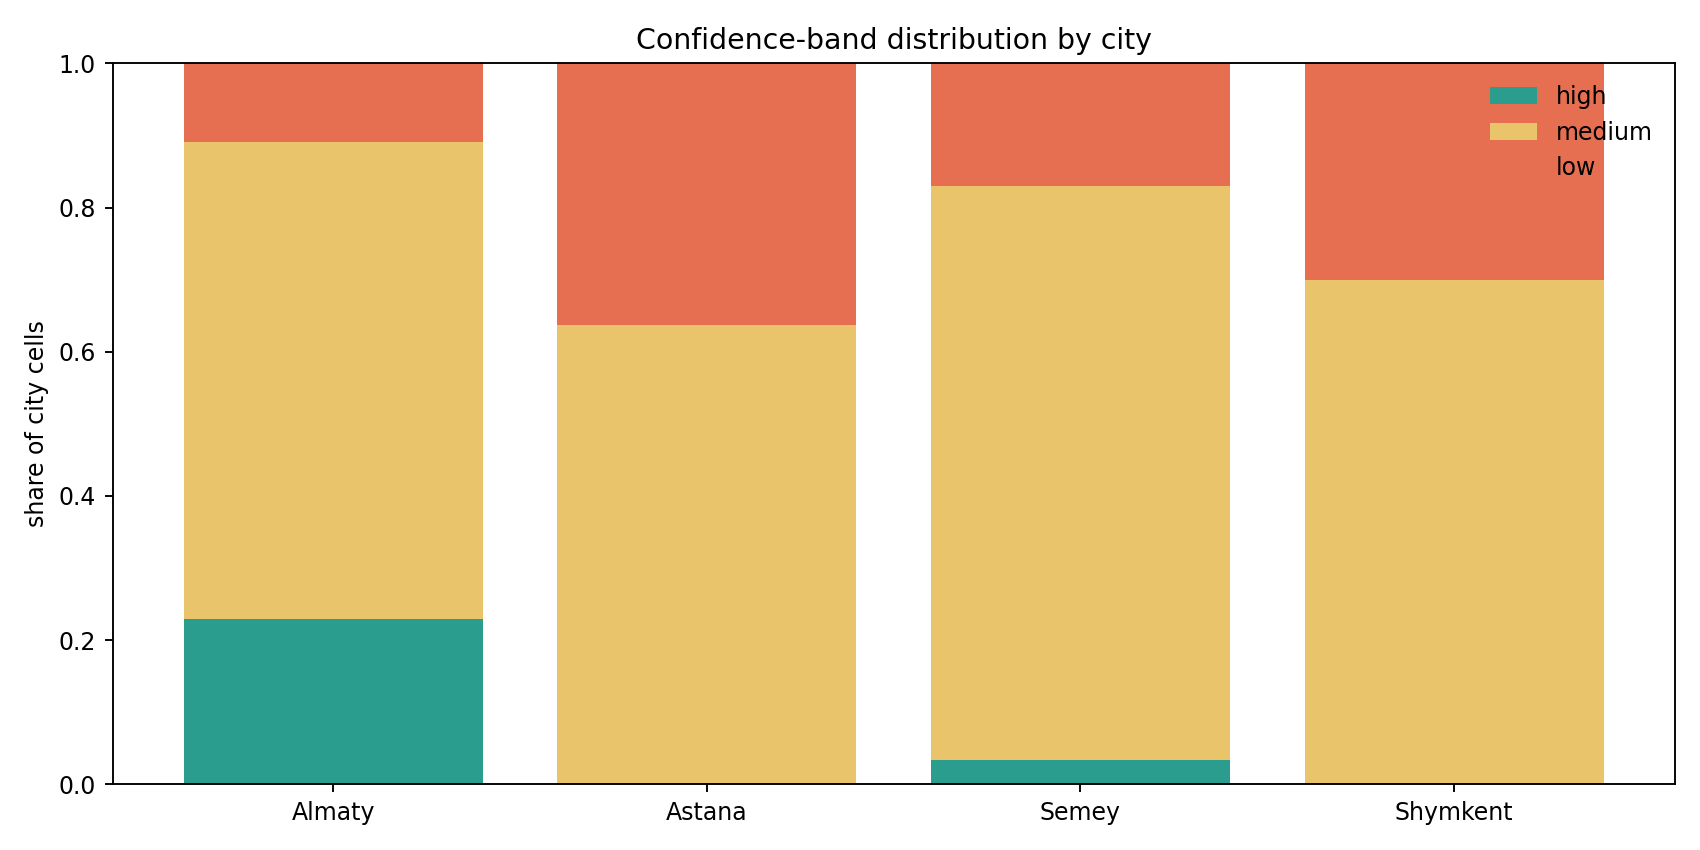
\includegraphics[width=0.95\textwidth]{figures/fig3_confidence_band_distribution.png}
\caption{Confidence-band distribution by city. The figure highlights that Almaty retains the clearest high-confidence share, while Astana and Shymkent remain caution-heavier. Confidence bands summarize bounded interpretation support; they are not probabilities of correctness.}
\label{fig:confidence-distribution}
\end{figure}

\subsection{Hotspot prioritization}

Table~\ref{tab:hotspot-priority} and Figure~\ref{fig:hotspot-priority} translate the uncertainty layer into the main practical use case: hotspot prioritization. Almaty is the strongest screening case, with 212 \texttt{high\_value\_high\_confidence} cells and another 310 \texttt{medium\_value\_high\_confidence} cells. Semey is mixed: it contains some stable high-value cells, but also a much larger caution-heavy component. Astana and Shymkent are dominated by review-oriented classes, with almost no stable high-value hotspot support.

\input{tables_tex/table4_hotspot_prioritization_summary.tex}

\begin{figure}[H]
\centering
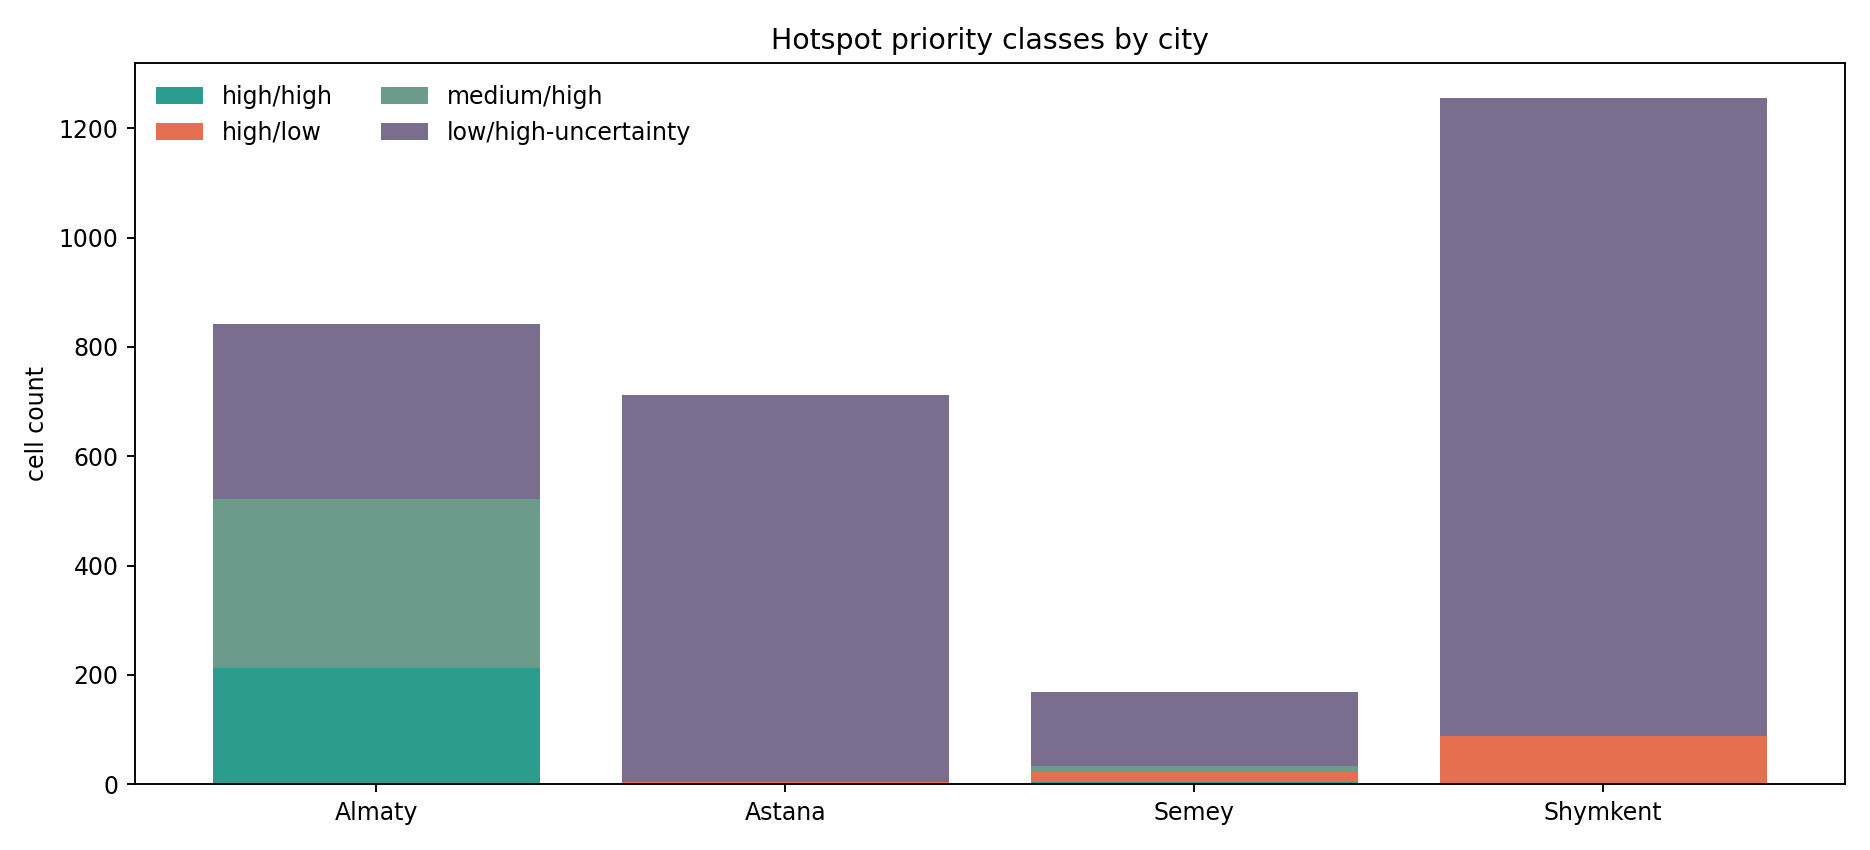
\includegraphics[width=0.95\textwidth]{figures/fig4_hotspot_prioritization_by_city.png}
\caption{Hotspot priority classes by city. Almaty concentrates the strongest stable hotspot support, whereas Astana and Shymkent are dominated by caution-oriented classes and should be used more conservatively. The classes are screening categories rather than verified population hotspot truth.}
\label{fig:hotspot-priority}
\end{figure}

This use-case framing is important for the paper's identity. City1 v3 is not trying to prove that its hotspot cells are administratively correct. It is trying to separate stronger and weaker screening candidates inside a calibrated proxy framework.

\subsection{Interval coverage and error alignment}

Table~\ref{tab:interval-coverage} summarizes interval coverage against proxy targets. Under the bounded LOCO-like protocol, coverage is weak in all four freeze cities, ranging from 0.294 in Shymkent to 0.403 in Semey. Under the inference-only proxy check, coverage is better but still mixed: 0.598 in Almaty, 0.613 in Astana, 0.692 in Semey, and 0.534 in Shymkent. These values support a cautious statement that the interval layer is informative but not uniformly tight.

\begin{table}[H]
\centering
\small
\caption{P10--P90 interval coverage against retained proxy targets. LOCO-like results come from the bounded local Phase 6 reconstruction setting; inference-only proxy checks come from the frozen four-city output package.}
\label{tab:interval-coverage}
\begin{tabular}{p{2.5cm}lrrrr}
\toprule
Protocol & City & Coverage & Below P10 & Above P90 & Median rel.\ unc. \\
\midrule
LOCO-like & Almaty   & 0.351 & 0.219 & 0.430 & 0.152 \\
LOCO-like & Astana   & 0.305 & 0.124 & 0.570 & 0.130 \\
LOCO-like & Semey    & 0.403 & 0.370 & 0.227 & 0.174 \\
LOCO-like & Shymkent & 0.294 & 0.541 & 0.165 & 0.151 \\
Inference-only proxy & Almaty   & 0.598 & 0.210 & 0.192 & 0.170 \\
Inference-only proxy & Astana   & 0.613 & 0.107 & 0.280 & 0.281 \\
Inference-only proxy & Semey    & 0.692 & 0.208 & 0.100 & 0.349 \\
Inference-only proxy & Shymkent & 0.534 & 0.273 & 0.194 & 0.175 \\
\bottomrule
\end{tabular}
\end{table}


Table~\ref{tab:error-alignment} and Figure~\ref{fig:validation-summary} show that the strongest positive alignment signal comes from uncertainty width itself. Spearman correlations between proxy-target error and uncertainty width are positive in every retained city/protocol combination, from 0.689 to 0.886. By contrast, relative-uncertainty ordering and confidence ordering are mixed, which is why v3 should be described as a bounded interpretation layer rather than a fully validated uncertainty model.

\input{tables_tex/table3_error_uncertainty_alignment.tex}

\begin{figure}[H]
\centering
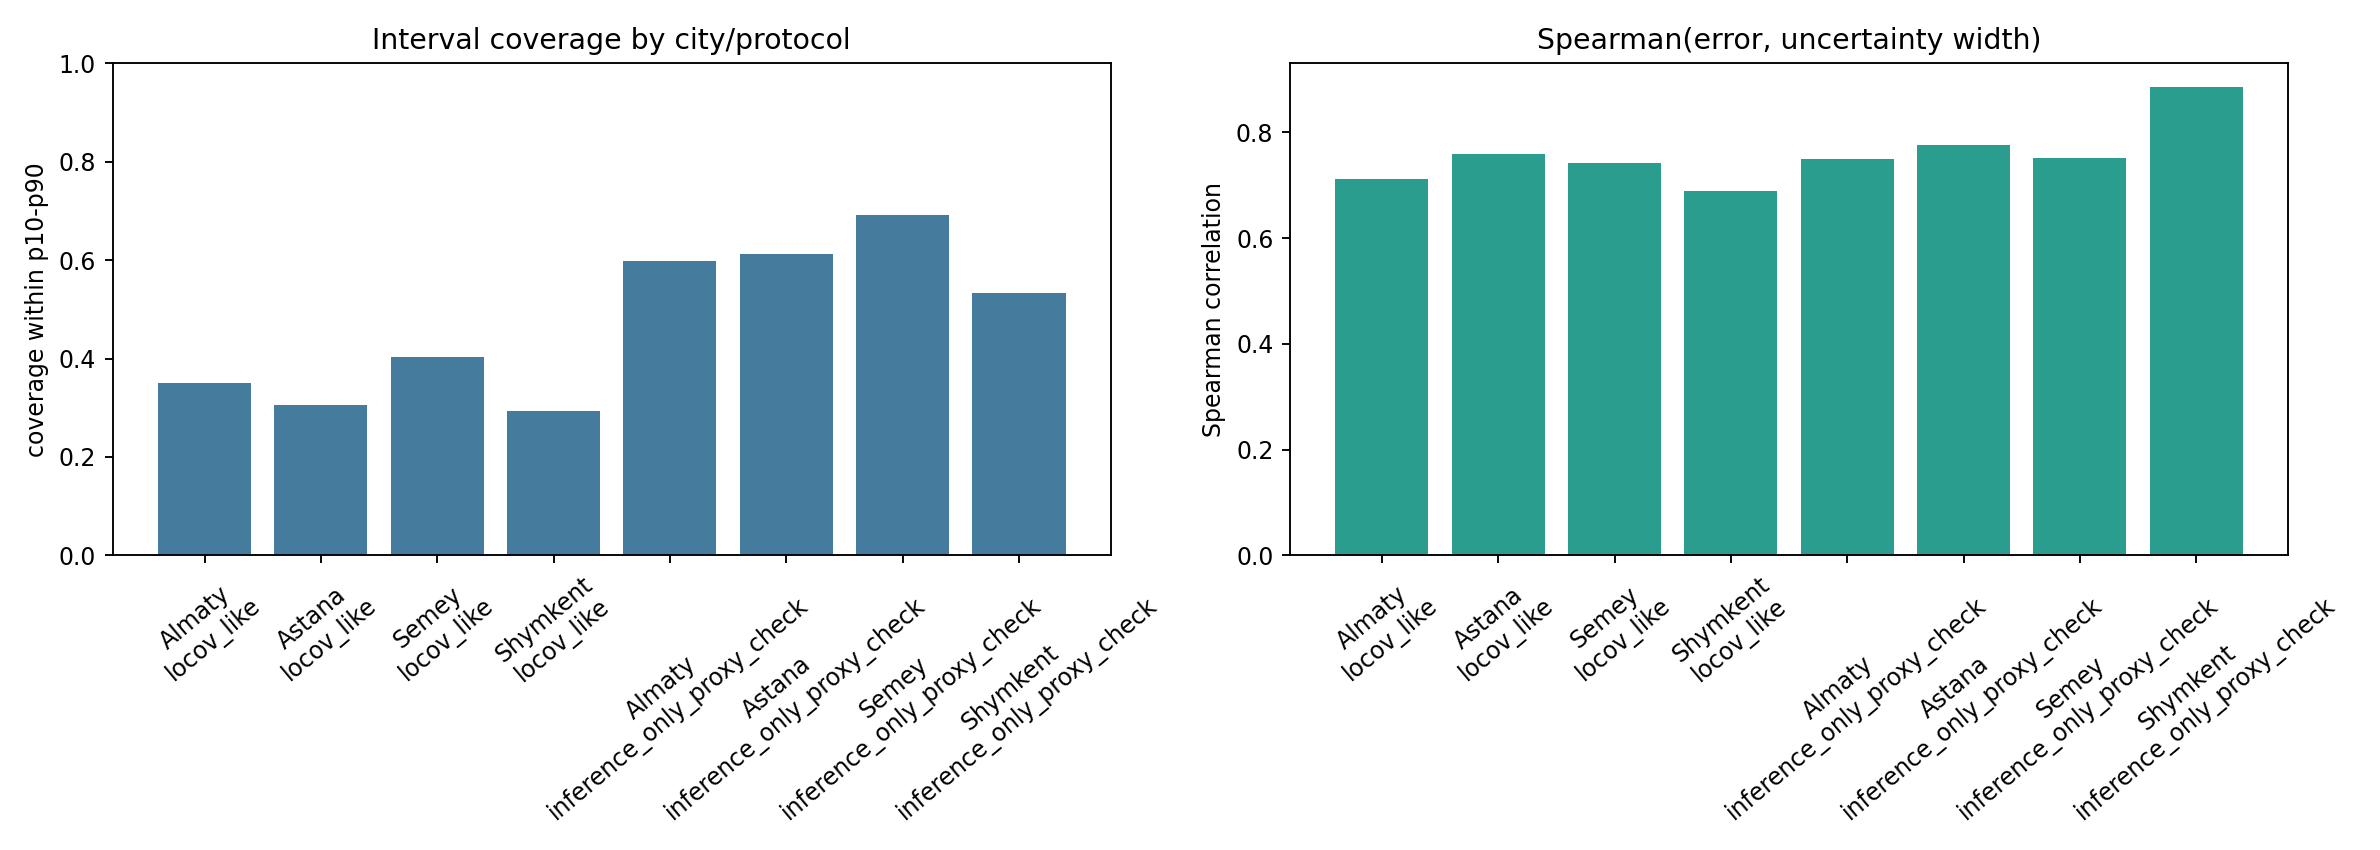
\includegraphics[width=\textwidth]{figures/fig5_uncertainty_validation_summary.png}
\caption{Summary of interval coverage and error-width alignment. Coverage is mixed across protocols, but uncertainty width tracks proxy-target error positively in all frozen city/protocol combinations shown here. This supports bounded usefulness of the interval layer without implying full uncertainty validation.}
\label{fig:validation-summary}
\end{figure}

\subsection{Confidence bands and hotspot stability}

Confidence-band behavior is summarized in Table~\ref{tab:confidence-bands}. In every city where a high band exists, it carries lower median relative uncertainty than the corresponding low band. Almaty shows the clearest separation, from 0.044 in the high band to 0.396 in the low band. Semey also shows strong uncertainty-burden separation, from 0.061 in the high band to 0.593 in the low band, even though its overall screening position remains mixed.

\begin{table}[H]
\centering
\small
\caption{Confidence-band summary. Shares are reported as percentages of city cells, and hotspot-priority share is the proportion of cells in each band that fall into one of the frozen priority classes.}
\label{tab:confidence-bands}
\begin{tabular}{llrrrrr}
\toprule
City & Band & Share (\%) & Median rel.\ unc. & Mean width & Mean error & Priority share \\
\midrule
Almaty   & high   & 22.9 & 0.044 & 62.59  & 58.57 & 0.740 \\
Almaty   & medium & 66.2 & 0.190 & 101.11 & 30.23 & 0.000 \\
Almaty   & low    & 10.9 & 0.396 & 69.12  & 32.09 & 0.952 \\
Astana   & medium & 63.7 & 0.217 & 92.02  & 35.06 & 0.000 \\
Astana   & low    & 36.3 & 0.423 & 122.08 & 41.65 & 0.565 \\
Semey    & high   & 3.4  & 0.061 & 35.17  & 73.73 & 0.400 \\
Semey    & medium & 79.7 & 0.316 & 93.09  & 21.21 & 0.000 \\
Semey    & low    & 16.9 & 0.593 & 97.39  & 20.86 & 0.886 \\
Shymkent & medium & 69.9 & 0.119 & 31.37  & 13.08 & 0.000 \\
Shymkent & low    & 30.1 & 0.308 & 24.82  & 9.03  & 0.845 \\
\bottomrule
\end{tabular}
\end{table}



The strongest reviewer-facing evidence appears in hotspot stability. Table~\ref{tab:hotspot-stability} and Figure~\ref{fig:hotspot-stability} show that stable classes such as \texttt{high\_value\_high\_confidence} and \texttt{medium\_value\_high\_confidence} have much higher mean stability metrics than caution-heavy classes. For example, Almaty's stable classes are near 0.777--0.784, Semey's stable classes are near 0.825--0.834, while caution-heavy classes mostly fall around 0.176--0.292. This is the clearest evidence that the uncertainty layer is doing useful screening work rather than adding decorative columns.

\input{tables_tex/table7_hotspot_stability_summary.tex}

\begin{figure}[H]
\centering
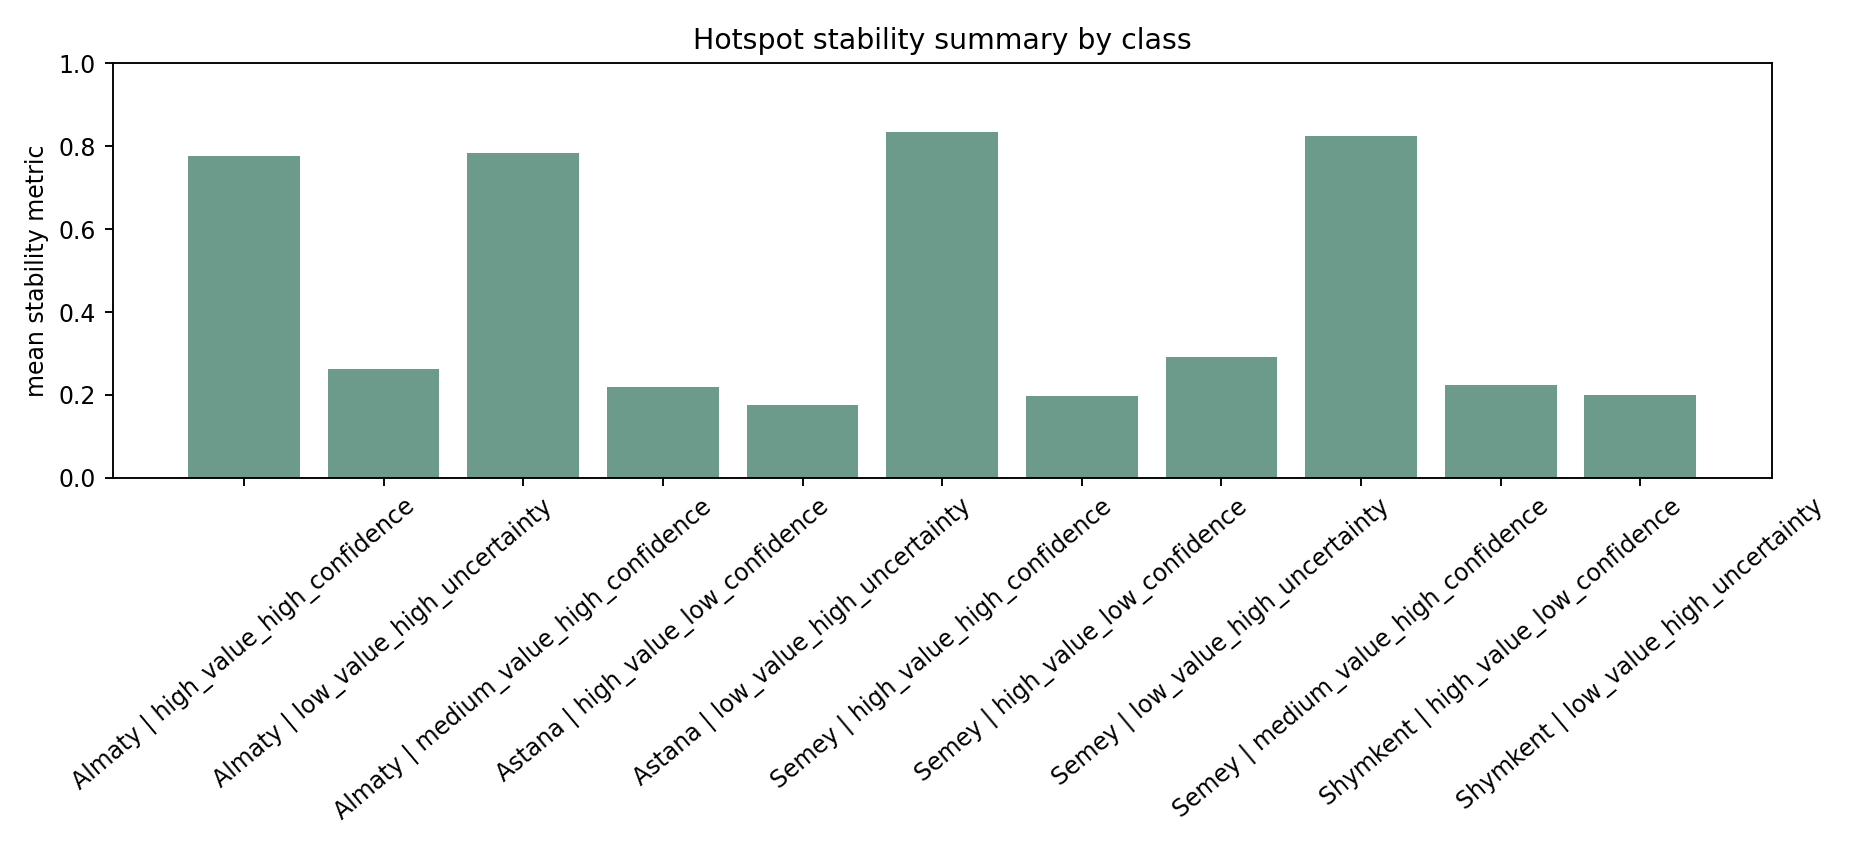
\includegraphics[width=\textwidth]{figures/fig6_hotspot_stability_summary.png}
\caption{Hotspot stability summary by class. Stable screening classes retain substantially higher mean stability than caution-heavy classes across the frozen city set. This is the strongest evidence layer for v3, but it still supports screening reliability rather than definitive population allocation.}
\label{fig:hotspot-stability}
\end{figure}

\subsection{District and external evidence}

Table~\ref{tab:district-external} collects the least supportive but still important evidence layers. District interval coverage remains partial because the frozen light package does not contain the offline district polygon/cell assignment artifacts needed for full p10/p50/p90 district-interval testing. What remains is partial after-aggregation support for Almaty, Astana, and Shymkent. External disagreement alignment against WorldPop and GHS-POP is mixed or negative, with Spearman correlations between disagreement and uncertainty ranging from $-0.188$ to $-0.494$ in the frozen table.

\input{tables_tex/table6_district_external_limitations_summary.tex}

These results are limitations, not fatal flaws. They mean that v3 cannot claim that uncertainty always rises where the surface disagrees more strongly with external products, and cannot claim that district interval coverage is solved. The manuscript therefore treats both layers as bounded contextual evidence rather than headline validation.

